\documentclass[10pt, compress]{beamer}
\usetheme[conference=MST1-GPM17,venue=Culham, date=14/11/2017, titleprogressbar, logo=RFX-logo]{Eurof}
\usepackage{listings,amsmath,multimedia, amssymb}
\usepackage{../beamerclass/tangocolors}
\usepackage{../beamerclass/rfxcolor}
% for drawing
\usepackage{pgf}
\usepackage{tikz}
\usetikzlibrary{arrows,shapes,backgrounds}
\usepackage{../beamerclass/onimage}
\usepackage[export]{adjustbox}
\usepackage{bm}
% for font
\usepackage[absolute,overlay]{textpos}
  \setlength{\TPHorizModule}{1mm}
  \setlength{\TPVertModule}{1mm}

\usepackage[style=nature,citestyle=authoryear-comp,defernumbers=true,maxnames=2,firstinits=true,
uniquename=init,backend=bibtex8,arxiv=abs,mcite]{biblatex}
\bibliography{biblio}
\renewcommand*{\bibfont}{\footnotesize}
\renewcommand*{\citesetup}{\footnotesize}
\usepackage[export]{adjustbox}
\makeatother
\mode<presentation>
\makeatletter
% add a macro that saves its argument
\newcommand{\footlineextra}[1]{\gdef\insertfootlineextra{#1}}
\newbox\footlineextrabox
% for reducing font on a single slide
\newcommand\Fontvi{\fontsize{8}{7.2}\selectfont}
\title{{\small Filamentary transport in high-power H-mode conditions and in
  no/small-ELM regimes to predict heat and particle loads on PFCs for
  future devices}}
\date{{\footnotesize 14 November 2017}}
\author[N. Vianello and V. Naulin]{N. Vianello, V. Naulin for Topic-21
Scientific Team}
\begin{document}
\tikzstyle{every picture}+=[remember picture]
\maketitle
\begin{frame}{Scientific Team}
\begin{center}
  Jiri Adamek, Matteo Agostini, Diogo Aguiam, Scott Allan, Matthias Bernert, Daniel Carralero Ortiz, 
Stefan Costea, Istvan Cziegler, Hugo De Oliveira, Joaquin Galdon-Quiroga, Gustavo Grenfell, Antti Hakola, 
Codrina Ionita-Schrittwieser, Heinz Isliker, Alexander Karpushov, Jernej Kovacic, Benoît Labit, Florian Laggner, Jens Madsen, 
Roberto Maurizio, Ken McClements, Fulvio Militello, Jeppe Miki Busk Olsen, Jens Juul Rasmussen, Timo Ravensbergen, Bernd Sebastian Schneider, Roman Schrittwieser, Jakub Seidl, Monica Spolaore, Christian Theiler, Cedric Kar-Wai Tsui, Kevin Verhaegh, Jose Vicente, 
Nickolas Walkden, Zhang Wei, Elisabeth Wolfrum
\end{center}
\end{frame}

\begin{frame}{2017 Top Objectives 
    12.12.2016}
  \Fontvi
\vspace{-1cm}
Deliverables listed during the call for manning of last December 
\begin{enumerate}
\item \only<2>{\color{ta3chameleon}} Cross-machine L-Mode
  shoulder dependence on current both at constant B$_t$ and at
  constant $q_{95}$. Rationale: disentangle the effect of current and
  parallel connection length
\item \only<2>{\color{taorange}}Establish robust scenario for density
  shoulder profile in H-Mode and establish dependence on
  fuelling/neutral profiles/divertor conditioon
\item \only<2>{\color{ta3chameleon}}Use the new HHF probe on AUG to study
  filamentary transport under high-power H-Mode conditions \only<2>{\color{consorziored}}and under
  different plasma configurations (SN, DN)
\item \only<2>{\color{taorange}}Study the role of ELM regimes,  neutral
  compression and particle density in filamentary transport and
  related shoulder formation
\item \only<2>{\color{taorange}} Identify the contribution of
  collisionality and seeding on filamentary transport and related
  shoulder formation
\item \only<2>{\color{consorziored}}Determine the effect of filaments and
  shoulder formation on target heat loads in different H-mode plasmas
\end{enumerate}
\onslide<2>{
  So far H-Mode operation has been limited to AUG since no operational
  scenario in high-density NBH heated plasma on TCV has been established
}
\end{frame}

\begin{frame}{L-Mode analysis: I$_p$ scan at constant q$_{95}$}
\Fontvi
  \vspace{-1cm}
  \begin{columns}    
  \begin{column}{0.65\textwidth}
    \centering{\includegraphics<1>[height=.8\textheight]{../../Experiments/AUG/analysis/pdfbox/EquilibraLparallelConstantQ95}}
    \includegraphics<2>[height=.81\textheight]{../../Experiments/AUG/analysis/pdfbox/GeneralIpScanConstantq95}
    \centering{\includegraphics<3>[height=.85\textheight]{../../Experiments/TCV/analysis/pdfbox/EquilibriaLparallelConstantQ95}}
    \centering{\includegraphics<4>[width=\textwidth]{../../Experiments/TCV/analysis/pdfbox/CurrentScanConstantQ95}}
    \centering{\includegraphics<5>[width=\textwidth]{../../Experiments/AUG/analysis/pdfbox/IpConstantQ95_Profiles_UsDiv}}
    \centering{\includegraphics<6>[width=\textwidth]{../../Experiments/AUG/analysis/pdfbox/n0_CurrentScanConstantQ95}}
    \centering{\includegraphics<7>[width=.6\textheight]{../../Experiments/AUG/analysis/pdfbox/RadiationPeakDensityIpScan_constantQ95}}
    \centering{\includegraphics<8>[width=\textwidth]{../../Experiments/TCV/analysis/pdfbox/IpConstantq95_samedensity}}
    \centering{\includegraphics<9>[width=\textwidth]{../../Experiments/TCV/analysis/pdfbox/CompareTargetProfilesConstantQ95}}
    \centering{\includegraphics<10>[width=\textwidth]{../../Experiments/AUG/analysis/pdfbox/BlobSizeCurrentScanConstantQ95}}
    \centering{\includegraphics<11>[width=\textwidth]{../../Experiments/AUG/analysis/pdfbox/GPI_blobs_AUG}}
    \centering{\includegraphics<12>[width=\textwidth]{../../Experiments/TCV/analysis/pdfbox/LambdaSizeIpScanConstantQ95}}
    
  \end{column}
  \begin{column}{0.35\textwidth}
    \begin{itemize}
      \item<1|only@1> AUG: All the shots were performed in the so-called
        Edge Optmized Configuration (EOC) shape. 
      \item<1|only@1> AUG: We matched correctly the shape and the L$_{\parallel}$
        here shown from outer divertor plate up to X-point 
      \item<2|only@2> AUG: The scan was performed with similar puffing
        rates for intermediate and higher current (0.8-1
        MA) whereas we reduced it at lower current to avoid early
        disruption
      \item<2|only@2> AUG: The total power (Ohmic plus NBI) was kept
        constant throughout the scan
      \item<2|only@2> AUG: We have comparable edge density, divertor neutral
        pressure and divertor temperature
      \item<3|only@3> TCV: We repeat the same excercise at TCV with a
        slight difference in the profile of parallel connection
        length. This required operation at unusual low toroidal field
        (up to 0.8T)
      \item<4|only@4> TCV: no additional heating
        has been used. Nevertheless the difference in power crossing the separatrix
        is small
      \item<4|only@4> TCV: The difference in target pressure similar
        to AUG behavior. 
      \item<5|only@5> AUG: At comparable edge density Upstream profiles are
        different with the tendency to develop shoulder easier at
        lower current. \alert{We have flattening of the upstream
          profiles only when $\Lambda_{div}$ is well above one on all
          the profile}
      \item<6|only@6> AUG: Neutrals estimated using calibrated D$_{\alpha}$
        cameras coupled with values of density and temperature at the
        target suggest a larger neutral density at lower current (even
        with comparable values of edge electron density)
      \item<7|only@7> AUG: At all the current a clear roll-over in
        peak density observed and we can also track the radiation
        front move away from target earlier in density at lower current
      \item<8|only@8> TCV: This tendency is not observed for TCV where
        profiles seem resilient to modification of Bt even though we
        reached pretty high value of $\Lambda_{div}$ all along the profile.
      \item<9|only@9> TCV: This is due to the fact that we can't
        observed during the density ramp any signature of rollover or detachment,
        \alert{whereas upstream profile modification at TCV are only observed
        well after rollover}
      \item<10|only@10> AUG: There is the tendency towards larger blobs
        at lower current at all values of $\Lambda_{div}$
      \item<11|only@11> AUG: This need to be further confirmed
        independently by GPI measurements. The present setup allows
        for space resolution of the order of mm with a 397 kframe/s
        sampling rate. Small amount of He gas flux needed ($\sim
        1.5e^{17} atoms/ms$)
      \item<12|only@12> TCV: this is not confirmed for TCV where blob
        sizes is rather constant over a rather large range of
        $\Lambda_{div}$. At the same time we do not observe target
        density rollover neither upstream profile flattening 
      \end{itemize}
    \end{column}
\end{columns}
\end{frame}

\begin{frame}{L-Mode analysis: I$_p$ scan at constant B$_{t}$}
\Fontvi
  \vspace{-1cm}
  \begin{columns}    
  \begin{column}{0.65\textwidth}
    \centering{\includegraphics<1>[height=.8\textheight]{../../Experiments/AUG/analysis/pdfbox/EquilibraLparallelConstantBt}}
    \centering{\includegraphics<2>[height=.8\textheight]{../../Experiments/AUG/analysis/pdfbox/GeneralIpScanConstantBt}}
    \centering{\includegraphics<3>[height=.85\textheight]{../../Experiments/TCV/analysis/pdfbox/EquilibriaLparallelConstantBt}}
    \centering{\includegraphics<4>[width=\textwidth]{../../Experiments/TCV/analysis/pdfbox/CurrentScanConstantBt}}
    \centering{\includegraphics<5>[width=\textwidth]{../../Experiments/AUG/analysis/pdfbox/IpConstantBt_Profiles_UsDiv}}
    \centering{\includegraphics<6>[width=\textwidth]{../../Experiments/AUG/analysis/pdfbox/n0_CurrentScanConstantBt}}
    \centering{\includegraphics<7>[width=.65\textheight]{../../Experiments/AUG/analysis/pdfbox/RadiationPeakDensityIpScan_constantBT}}
    \centering{\includegraphics<8>[width=\textwidth]{../../Experiments/TCV/analysis/pdfbox/IpConstantBt_samedensity}}
    \centering{\includegraphics<9>[width=\textwidth]{../../Experiments/TCV/analysis/pdfbox/CompareTargetProfilesConstantBt}}
    \centering{\includegraphics<10>[width=\textwidth]{../../Experiments/AUG/analysis/pdfbox/BlobSizeCurrentScanConstantBT}}
    \centering{\includegraphics<11>[width=\textwidth]{../../Experiments/TCV/analysis/pdfbox/LambdaSizeIpScanConstantBt}}
    
  \end{column}
  \begin{column}{0.35\textwidth}
    \begin{itemize}
      \item<1|only@1> AUG: We matched correctly the shape the parallel
        connection length L$_{\parallel}$ is modified consistently
      \item<1|only@1> AUG: The scan was performed with similar puffing rate (0.8-1
        MA) whereas we reduced it at lower current to avoid early disruption
      \item<2|only@2> AUG: We have comparable edge density and divertor neutral
        pressure even though pressure increase earlier at higher current
      \item<2|only@2> AUG: The total power (Ohmic plus NBI) was kept
        constant throughout the scan
      \item<3|only@3> TCV: We repeat the same excercise at TCV with a
        consistent variation of parallel connection length
      \item<4|only@4> TCV: no additional heating
        used. Nevertheless the difference in power crossing the separatrix
        is small
      \item<4|only@4> TCV: Neutral compression is roughly constant between
      \item<5|only@5> AUG: At comparable edge density Upstream profiles are
        different with the tendency to develop shoulder easier at
        lower current. \alert{We have flattening of the upstream
          profiles only when $\Lambda_{div}$ is well above one on all
          the profile}
        \item<6|only@6> Neutrals at lower current are substantially
          higher even with similar edge density profiles.
        \item<7|only@7> Neutrals at lower current are substantially
          higher even with similar edge density profiles.
      \item<8|only@8> TCV: This tendency is substantially confirmed at
        TCV where
        profiles  
      \item<9|only@9> TCV: This is consistent with onset of detachment
        (at least in intermediate and lower current)
      \item<10|only@10> AUG: While the general observation of increasing
        blob size with $\Lambda_{div}$ is confirmed there are no
        differences between the current
      \item<11|only@11> TCV: confirm the observation of AUG. 
      \end{itemize}
    \end{column}
\end{columns}
\end{frame}

\begin{frame}{LSN \textit{vs} Double null on TCV}
%  \begin{columns}
%    \begin{column}{0.5\textwidth}
      \centering{\includegraphics<1>[width=.6\textwidth]{../../Experiments/TCV/analysis/pdfbox/CompareTargetProfilesLSN-DN}}
      \centering{\includegraphics<2>[width=.8\textwidth]{../../Experiments/TCV/analysis/pdfbox/DNRadiation_58623}}
      \centering{\includegraphics<3>[width=.8\textwidth]{../../Experiments/TCV/analysis/pdfbox/DNRadiation_58624}}
      \centering{\includegraphics<4>[width=.8\textwidth]{../../Experiments/TCV/analysis/pdfbox/LambdaSizeLSN-DN}}
%    \end{column}
%    \begin{column}{0.5\textwidth}
      \begin{itemize}
        \item<1|only@1> Comparing similar L-Mode density ramp at same
          current in LSN and DN with ion $\mathbf{B}\times\nabla B$
          pointing towards the floor. Lower ion flux to lower target
          observed in DN and profiles before rollover seem more broad
          in LSN. After rollover the profiles are actually similar
      \item<2|only@2>  From bolometry we can observe an
          unbalanced movement of the radiation front suggesting a non
          perfectly balanced DN
      \item<3|only@3> This is confirmed at higher current where the
        more active X-point is the upper one with a consequent higher
        radiation from bolometry chords    
      \end{itemize}
%    \end{column}
%  \end{columns}
\end{frame} 

\begin{frame}{H-Mode investigation: puffing location}
\Fontvi
  \vspace{-1cm}
\begin{columns}
  \begin{column}{0.65\textwidth}
    \centering{\includegraphics<1>[height=0.85\textheight]{../../Experiments/AUG/analysis/pdfbox/PuffingLocation}}
    \centering{\includegraphics<2>[width=\textwidth]{../../Experiments/AUG/analysis/pdfbox/CompareShot34276_34277}}
    \only<3>{
      \begin{tikzonimage}[width=\textwidth]{../../Experiments/AUG/analysis/pdfbox/EvolutionEdgeProfiles_34276_34277}
        \draw [->, ultra thick, white] (0.2, 0.45) -- (0.3, 0.55);
        \draw [->, ultra thick, white] (0.62, 0.45) -- (0.72, 0.55);
      \end{tikzonimage}   
    }
  \end{column}
  \begin{column}{0.35\textwidth}
    \begin{itemize}
      \item<1-> Similar puff from Lower and Upper divertor valves
        (\alert{we asked for divertor/midplane valves})
      \item<2-> Discharge with a total amount 6.5 heating power
        with equivalent behavior also in the lower divertor
        independently from the puffing location
      \item<3-> Edge density profiles from Li-Beam evolution are
        pretty similar
      \item<3|alert@3> Similar behavior observed from RIC Antenna 4
        for the available shot
    \end{itemize}
  \end{column}
\end{columns}
\end{frame}

\begin{frame}{Compare fueling with/without cryopumps}
\Fontvi
  \vspace{-1cm}
\begin{columns}
  \begin{column}{0.65\textwidth}
    \centering{\includegraphics<1>[width=\textwidth]{../../Experiments/AUG/analysis/pdfbox/CompareShot34276_34278}}
    \centering{\includegraphics<2>[height=.65\textheight]{../../Experiments/AUG/analysis/pdfbox/PuffingIpolsola34276_34278}}
    \only<3>{
    \begin{tikzonimage}[width=\textwidth]{../../Experiments/AUG/analysis/pdfbox/EvolutionEdgeProfiles_34276_34278}
      \draw [->, ultra thick, white] (0.2, 0.45) -- (0.3, 0.55);
      \draw [->, ultra thick, dashed, red] (0.62, 0.45) -- (0.72, 0.55);
    \end{tikzonimage}}
  \centering{\includegraphics<4>[height=.85\textheight]{../../Experiments/AUG/analysis/pdfbox/Shot_34276_34278_InterELMprofiles}}
  \end{column}
  \begin{column}{0.35\textwidth}
    \begin{itemize}
    \item<1-> Same fueling but with cryo-pumps
      \item<1-> H-5 density is different and remain constant, both
        divertor and midplane pressure are reduced (to 1/3
        approximately) no sign of detachment
      \item<2-> Different ELMy regimes reached with reduced size and
        increased frequency without the cryopumps
      \item<3-> Also with this amount of fueling weaker indication of SOL
        saturation observed as confirmed by Li-Beam and by RIC (Antenna 4)
      \item<4> Inter-ELM resolved profile suggest a flattening even
        with the cryompumps still even though $\Lambda_{div}$ is
        marginal above 1 only in the near SOL
        
    \end{itemize}
  \end{column}
\end{columns}
\end{frame}

\begin{frame}{Matching scenarios with cryo-pumps}
\Fontvi
  \vspace{-1cm}
\begin{columns}
  \begin{column}{0.65\textwidth}
    \centering{\includegraphics<1>[width=\textwidth]{../../Experiments/AUG/analysis/pdfbox/CompareShot34276_34281}}
    \centering{\includegraphics<2>[width=\textwidth]{../../Experiments/AUG/analysis/pdfbox/PuffingIpolsola34276_34281}}
    \centering{\includegraphics<3>[width=\textwidth]{../../Experiments/AUG/analysis/pdfbox/EvolutionEdgeProfiles_34276_34281}}
    \centering{\includegraphics<4>[height=0.9\textheight]{../../Experiments/AUG/analysis/pdfbox/Shot_34278_34281_InterELMprofiles}}
    \centering{\includegraphics<5>[height=0.9\textheight]{../../Experiments/AUG/analysis/pdfbox/CompareCas34278_34281}}
  \end{column}
  \begin{column}{0.35\textwidth}
    \begin{itemize}
      \item<1-> To match similar edge density and divertor pressure
        and to reach the same level of detachment we increase the
        fueling by almost a factor of 3, increasing also the rate. In
        addition to that we also increase substantially the N
        puffing. \alert{Degraded H-Mode reached earlier in density
          without the cryopumps}
      \item<2-> Similar ELMy behavior obtained during the density ramp  
      \item<3-> Now the scenario suggest a strong profile flattening
        even with the cryopumps
       \item<4-> Inter-ELM resolved Li-Be profiles confirm this with
         shoulder formed with similar strength even with the cryopumps
         in operation.
         \item<5> We can also confirm that additional fueling change
           substantially the blob size which increases consistently
           with the modification of $\Lambda_{div}$
    \end{itemize}
  \end{column}
\end{columns}
\end{frame}

\begin{frame}{Fast electron generation}
\Fontvi
  \begin{columns}
    \begin{column}{0.5\textwidth}
      \centering{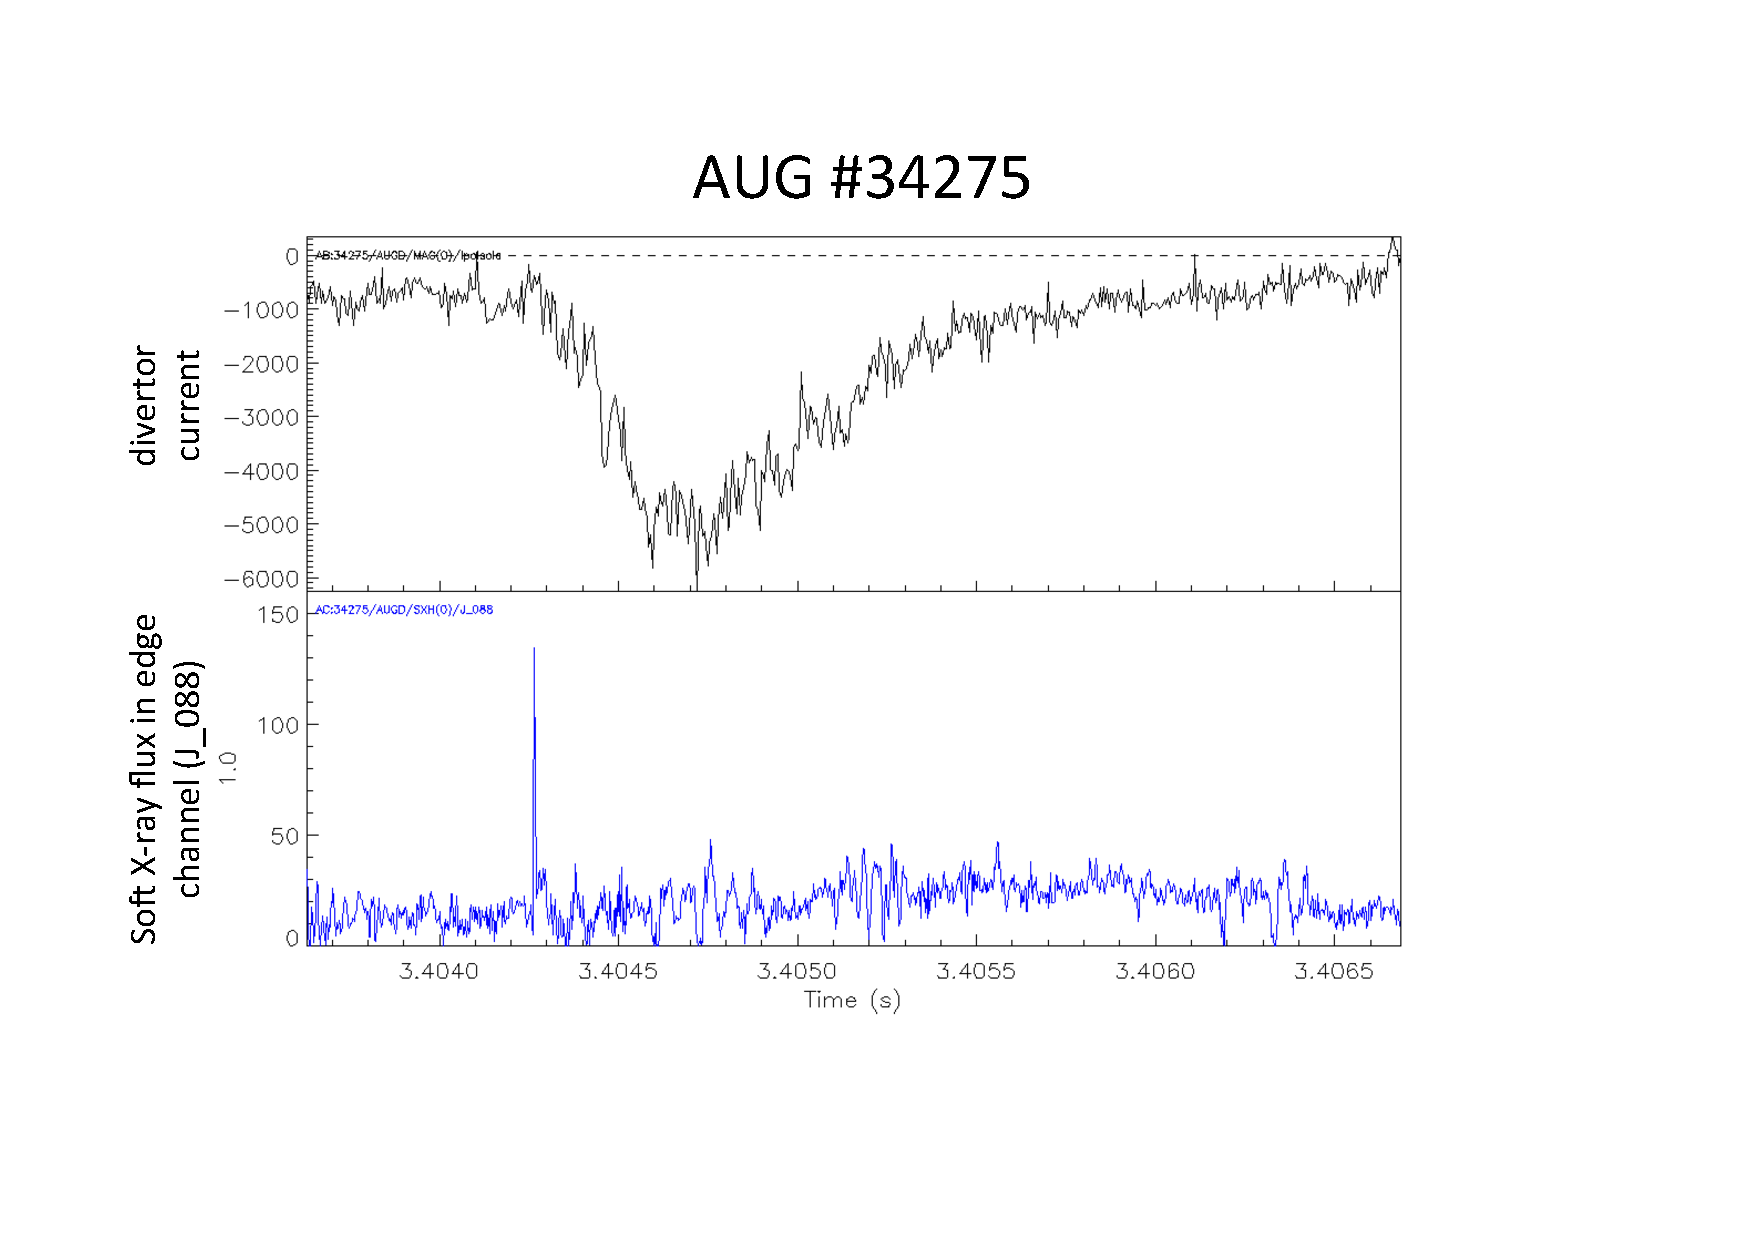
\includegraphics[width=\textwidth]{../../Experiments/AUG/analysis/pdfbox/SXR_ken}}
    \end{column}
    \begin{column}{0.5\textwidth}
\begin{itemize}
      \item Bursts of nonthermal 2nd harmonic electron cyclotron emission and edge soft X-ray emission often occur at start of ELM filament eruption in low collisionality AUG pulses – evidence of filament reconnection
\item Soft X-ray bursts were seen at start of ELM filament eruption in T21-AUG pulses, but not ECE bursts, probably due to higher collisionality in these pulses
\item Peak nonthermal ECE emission appears to originate from top of pedestal
\item Work is ongoing to determine conditions for occurrence of ECE \& SXR bursts, e.g. in terms of pedestal collisionality – there is no clear correlation between ELM size \& SXR flux
\end{itemize}
\end{column}

  \end{columns}
\end{frame}

\begin{frame}{Comments on difficulties for H-Mode in TCV}

\end{frame}
\begin{frame}{Comments on different divertor geometry which can be explored}

\end{frame}

\begin{frame}{Program for 2018: AUG}
  \begin{itemize}
     \item X-point manipulator (hopefully with NPH) triggered at
	the same time as MPM
     \item X-point vertical shift in order to have SP at different
	vertical heigth at the target. \alert{This could suggest us if
        similar behavior as the one observed on JET are visible at AUG}
     \item DN discharges. With slow movement of the second X-point into the vessel
	to be performed at constant power/density where shoulder
        alreay exists. \alert{This is mandatory to complement the
          information obtained on TCV}
     \item USN with midplane/X-point manipulator to monitor the upstream SOL 
\end{itemize}
 \end{frame}

\begin{frame}{Program for 2018: TCV}
  \begin{itemize}
     \item H-Mode ?
      \item Long divertor legs (probe in the lower port)
      \item SnowFlake to monitor the fluctuations in between the 2 separatrix
	to be done in high density discharges
       \item Try to move the second X-point in SN divertor at a different
	Z position while keeping the same radial distances between the
	points
\end{itemize}
\end{frame}

\begin{frame}{Program for 2018: MAST-U}
  \begin{itemize}
     \item Influence of neutral recycling source in establishing upstream profiles
	and comparison between Low-RT and Vertical target. Look also ath the heat
	loads
      \item Current scan at constant q95/constant Bt
      \end{itemize}
\end{frame}

%\begin{frame}{Outline}
% 	\begin{itemize}
% 		\item Background 
% 		\item Plans (we will not make a detailed list of the
%                   proposal, we already tried to combine and summarize them)
% 		\item Discussion
% 	\end{itemize}	
% \end{frame}

% \section{Background}
% \begin{frame}{Present status}
%   \setbeamercovered{transparent}
%   \begin{enumerate}[<+(1) | invisible@-+>]
%     \item Experimental and theoretical investigations suggest that SOL density profiles are
%       determined by the balance between radial filamentary transport and parallel dynamics
%     \item The balance changes at high density and leads to broadened SOL density profiles $\rightarrow$ \emph{shoulder formation}
%     \item This is observed in L-mode plasmas in a variety of devices including AUG \parencite{Carralero:2014gs},
%       TCV \parencite{Garcia:2007p2615} and MAST \parencite{Militello:2016hk}
%     \item Observations exhibit various other dependencies e.g., divertor
%       collisionality, plasma current, seeding. \alert{Results from
%         different devices not fully reconciled and the underlying mechanism is not fully understood.}
%     \item Studies of shoulder formation in H-Mode are so far limited 
% 	%\item Particle and energy transport in the SOL is crucial for lifetime of PFC in ITER and DEMO
% %    \item First we will report a summary of the achievements and then
%  %    personal comments and plans
%     \end{enumerate}
% \end{frame}
% \section{L-Mode}
% \begin{frame}{L-Mode studies: AUG/1}
%   \begin{columns}
%     \begin{column}{0.5\textwidth}
%       \begin{itemize}
%       \item<1-> AUG and JET \parencite{Carralero:2015gu} suggest that divertor collisionality 
%         \begin{equation*}
%         \Lambda_{div} = \frac{L_{\parallel}/c_s}{1/\nu_{ei}}\frac{\Omega_i}{\Omega_e}
%       \end{equation*}
%       controls filaments size
%         \item<2-> \textcolor{red}{Tested by changing n$_e$
%             and $T_e$ through fueling/seeding/heating}
%         \item<3-> This determines a change of the velocity-size
%           scaling from
%             \textcolor{ta3chameleon}{sheath-limited}
%         to \textcolor{blue}{inertial regime}.
%        \onslide<4->{\alert{$\Lambda_{div}$ rules the density profile scale
%            length}}
%        \item<5> This finally determines the shoulder formation
%         \end{itemize}
%     \end{column}
%     \begin{column}{0.5\textwidth}
%       \only<1-2>{
%       \begin{tikzonimage}[width=\textwidth]{../../pdfbox/KoM15Nov/CarraleroPRL15a}
%           \draw [thick, ta3chameleon, thick, rotate=1] (0.43,0.25) ellipse (0.23 and 0.1);
%           \draw [thick, blue, thick, rotate=-4] (0.8,0.55) ellipse (0.1 and 0.33);
%         \only<2>{
%           \draw [ultra thick, red, thick, dashed] (0.5,0.63) circle (0.12);
%         }
%       \end{tikzonimage}}
%     \only<3-4>{
%       \begin{tikzonimage}[width=\textwidth]{../../pdfbox/KoM15Nov/CarraleroPRL15b}
%           \draw [ultra thick, ta3chameleon, rotate=1] (0.2,0.5) ellipse (0.05 and 0.4);
%           \draw [thick, blue, rotate=15] (0.65,0.07) ellipse (0.4 and 0.1);
%       \end{tikzonimage}
%     }
%     \includegraphics<5>[width=\textwidth]{../../pdfbox/KoM15Nov/CarraleroPRL15c}
%     \end{column}
%   \end{columns}
% \end{frame}


% \begin{frame}{L-Mode studies: AUG/2}
%   \begin{columns}
%     \begin{column}{0.5\textwidth}
%       \begin{itemize}
%       \item<1-> Profile modified by an increase of blob-size and change of
%         \alert{packing fraction: $f_{fil} = \nu_{fil}\tau_{AC}$}
%         \onslide<2->{\textcolor{blue}{and filament relative density}
%           {\footnotesize (Carralero 2016 in preparation)}}
%       \item<3-> As a consequence the contribution of filaments to
%         radial transport increases
%       \item<4|only@4> \alert{Beware the change of frequency may be due to a
%         modification of fluctuation velocity which is known to vary
%         with densities ad normalized greenwald fraction \parencite{0029-5515-51-5-053020}}  
%       \item<5> Parallel flow is strongly reduced whenever we increase
%         the divertor collisionality
%       \end{itemize}
%     \end{column}
%       \begin{column}{0.5\textwidth}
%         \includegraphics<1>[width=\textwidth]{../../pdfbox/KoM15Nov/CarraleroMST16a}
%         \includegraphics<2>[width=\textwidth]{../../pdfbox/KoM15Nov/CarraleroMST16b}
%         \includegraphics<3>[width=\textwidth]{../../pdfbox/KoM15Nov/CarraleroMST16c}
%         \includegraphics<4>[width=\textwidth]{../../pdfbox/KoM15Nov/AgostiniNF2011}
%         \includegraphics<5>[width=\textwidth]{../../pdfbox/KoM15Nov/CarraleroMST16d}
%       \end{column}
%     \end{columns}
%   \end{frame}

%   \begin{frame}{L-Mode studies:AUG/3}
%   \begin{columns}
%     \begin{column}{0.5\textwidth}
%       \begin{itemize}
%       \item<1-> Electron and ions behave differently
%       \item<2|only@2> T$_{e, fil} \sim 1.2 $T$_{e, bk}$ roughly constant
%         accross the SOL and slightly affected by the increase of
%         divertor collisionality
%       \item<3|only@3> Ions are strongly affected: for
%         \textcolor{red}{$\Lambda_{div}<1$ T$_{i, fil} > $ T$_{i, bk}$
%           and $\lambda_{T_i} \sim 30$
%           mm}. \textcolor{blue}{$\Lambda_{div}>1$ T$_{i, fil} \sim $
%           T$_{i, bk}\sim 25$ eV
%           and $\lambda_{T_i} \sim 8$ mm}
%        \item<4-> Ion energy spectrum from
%          $\mathbf{E}\times\mathbf{B}$ analyzer shrinks towards lower
%          energy for $\Lambda_{div} > 1$
%        \item<5> EMC3-Eirene simulation suggests that such a reduction
%          can't be accounted for thermalization process. An
%          \alert{ionization front builds in front of the limiter shadow}   
%        \end{itemize}
%     \end{column}
%       \begin{column}{0.5\textwidth}
%         \includegraphics<2>[width=\textwidth]{../../pdfbox/KoM15Nov/CarraleroMST16e}
%         \includegraphics<3>[width=\textwidth]{../../pdfbox/KoM15Nov/CarraleroMST16f}
%         \includegraphics<4>[width=\textwidth]{../../pdfbox/KoM15Nov/CarraleroMST16g}
%         \includegraphics<5>[width=\textwidth]{../../pdfbox/KoM15Nov/CarraleroMST16h}
%       \end{column}
%     \end{columns}
%   \end{frame}

%   \begin{frame}{L-Mode: TCV}
%     \begin{columns}
%     \begin{column}{0.5\textwidth}
%       \begin{itemize}
%       \item<1|only@1> Flexibility has allowed to test $\Lambda_{div}$
%         dependence on L$_{\parallel}$ by varying flux expansion f$_x$:
%         \begin{equation*}
%           f_x = \frac{(B_p/B_t)_{MP}}{(B_p/B_t)_{SP}}
%         \end{equation*}
%         in ohmic density ramps \parencite{vianello:iaea2016}
%       \item<2|only@2> Slight variation of density profiles at the target but
%         due to direct dependence on L$_{\parallel}$ large increase of
%         $\Lambda_{div}$. \alert{Upstream profiles only varies whenever
%         we reach a certain amount of $\langle n_e \rangle$}
%        \only<3-5>{\item Weak dependence of blob-size from $\Lambda_{div}$,
%         \onslide<4-5>{\textcolor{red}{also on a statistical
%             basis}}. \onslide<5>{Strong dependence on average density,
%           independent of L$_{\parallel}$}}
%        \item<6|only@6> $\lambda_n$ depends clearly on blob-size
%          whereas the dependence on divertor condition is less
%          obvious. \alert{$\Lambda_{div}$ necessary but not sufficient}
%       \end{itemize}
%     \end{column}
%       \begin{column}{0.5\textwidth}
%         \includegraphics<2>[width=\textwidth]{../../pdfbox/KoM15Nov/VianelloIAEA16a}
%         \includegraphics<3>[width=\textwidth]{../../pdfbox/KoM15Nov/VianelloIAEA16b}
%         \includegraphics<4>[width=\textwidth]{../../pdfbox/KoM15Nov/VianelloIAEA16c}
%         \includegraphics<5>[width=\textwidth]{../../pdfbox/KoM15Nov/VianelloIAEA16d}
%         \includegraphics<6>[width=\textwidth]{../../pdfbox/KoM15Nov/VianelloIAEA16e}
%       \end{column}
%     \end{columns}
%   \end{frame}

%   \begin{frame}{L-Mode: JET}
%     \begin{columns}
%     \begin{column}{0.5\textwidth}
%       \begin{itemize}
%       \item<1|only@1> The shoulder formation strongly depends on
%         divertor geometry, disappear with vertical target and strike
%         point closest to cryogenics pumps \parencite{Wynn:EPS2016}
%       \item<2|only@2> The midplane pressure from baratrons is
%         equivalent between the different divertor. \alert{This would
%           indicate that SOL neutral density at the outboard midplane does not play any role}
%        \item<3|only@3> In the horizontal target configuration the
%          results indicate that the shoulder forms right at the
%          transition from sheath-limited to high-recycling where also
%          $\Lambda_{div}$ strongly increase
%        \item<4|only@4> Shoulder amplitude correlates with strike
%          points position. \alert{Shoulder, ionization and
%            $\Gamma_{ion, plate}$ larger when R$_{strike}$ smaller away
%          from the pump}
%        \item<5|only@5> In seeded discharges the transition observed at
%          very high level of $\Lambda_{div} >> 1$
%       \end{itemize}
%     \end{column}
%       \begin{column}{0.5\textwidth}
%         \includegraphics<1>[width=\textwidth]{../../pdfbox/KoM15Nov/LipschultzITPA16a}
%         \includegraphics<2>[width=\textwidth]{../../pdfbox/KoM15Nov/LipschultzITPA16b}
%         \includegraphics<3>[width=\textwidth]{../../pdfbox/KoM15Nov/LipschultzITPA16c}
%         \includegraphics<4>[width=\textwidth]{../../pdfbox/KoM15Nov/LipschultzITPA16d}
%         \includegraphics<5>[width=\textwidth]{../../pdfbox/KoM15Nov/LipschultzITPA16e}
%       \end{column}
%     \end{columns}
%   \end{frame}

%   \begin{frame}{L-Mode: MAST}
%     \begin{columns}
%     \begin{column}{0.5\textwidth}
%       \begin{itemize}
%       \item<1|only@1> Strong dependence on
%         I$_p$ \parencite{Militello:2016hk}. Increasing I$_p$ at
%         constant toroidal field shoulder disappears. Consistent with
%         observation in other devices
%       \item<2|only@2> Filaments binormal dimension increases with
%         current \parencite{Kirk:2016jj} or equivalently decreases with L$_{\parallel}$
%        \item<3|only@3> Filament radial velocity decreases with current
%          as well as the radial dimension \parencite{Kirk:2016jj}
%       \end{itemize}
%     \end{column}
%       \begin{column}{0.5\textwidth}
%         \includegraphics<1>[width=\textwidth]{../../pdfbox/KoM15Nov/MilitelloNF16a}
%         \includegraphics<2>[width=\textwidth]{../../pdfbox/KoM15Nov/KirkPPCF16a}
%         \includegraphics<3>[width=\textwidth]{../../pdfbox/KoM15Nov/KirkPPCF16c}
%       \end{column}
%     \end{columns}
%   \end{frame}

%   \section{H-Mode}
%   \begin{frame}{AUG: H-Mode}
%     \begin{columns}
%     \begin{column}{0.4\textwidth}
%       \begin{itemize}
%       \item<1|only@1> SOL profiles in H-Mode so far investigated on
%         AUG \parencite{Muller:2015jt,Sun:2015bu,carralero:psi2016}
%       \item<2|only@2> Differently from L-Mode, complete detachment
%         suggested to be mandatory for increasing of $\lambda_n$ \parencite{Sun:2015bu}
%        \item<3|only@3> In weak H-Mode \parencite{carralero:psi2016}
%          shoulder depends on a combination of $\Lambda_{div}$ and
%          fueling rate. Complete detachment seems instead not necessary
%          although very weak shoulder
%       \end{itemize}
%     \end{column}
%       \begin{column}{0.6\textwidth}
%         \includegraphics<1>[width=\textwidth]{../../pdfbox/KoM15Nov/MuellerJNM15a}
%         \includegraphics<2>[width=\textwidth]{../../pdfbox/KoM15Nov/SunPPCF15a}
%         \includegraphics<3>[width=\textwidth]{../../pdfbox/KoM15Nov/CarraleroMST16i}
%       \end{column}
%     \end{columns}
%   \end{frame}

%   \section{Open issues}
%   \begin{frame}{Open and unresolved issues}
%   \setbeamercovered{transparent}
%   \begin{enumerate}[<+(1) | invisible@-+>]
%     \item Does $\Lambda_{div}$ unify the picture among the devices?
%       \alert{No, does neutral pressure play a role?}
%     \item If neutrals play a role is it at the divertor and/or at the midplane?
%       \alert{Contradictory results if one include experiments with
%         midplane puffing, JET and EIRENE simulations}
%     \item Does L$_\parallel$ play any role? \alert{So far TCV suggests no
%       dependence from f$_x$ scan but both TCV and MAST observe an
%       I$_p$ dependence. MAST clearly state filament $\sigma_{\perp}$
%       increases with L$_{\parallel}$ }
%     \item Is cooling the divertor with fueling or seeding equivalent? \alert{Contradictory observations in AUG and JET}
%     \item Do we observe same behavior in L and H-Mode? \alert{So
%       far no as shown in H-Mode AUG. We need higher detachment
%       condition and we need enough fueling}
%       \item Is the density shoulder accompanied with an ion temperature shoulder?
% %      \item What are the underlying mechanisms? 
%     \end{enumerate}
%   \end{frame}
  
% \section{Topic 21 experiments }
% \begin{frame}{$n_{\text{proposed shots}} \gg n_{\text{allocated shots}}$}
% 	\begin{itemize}
% 		\item 15 were proposals submitted to Topic 21
% 		\item Proposals include experiments on all three machines 
% 		\item There are overlaps between several of the proposals 
% 		\item Preliminary shot allocation. AUG: 14. MAST: 13. TCV: 23 
% 		\item However, total number of proposed shots:  \textbf{449}
% 		\item Several of the proposed experiments can be combined. \underline{But we must prioritize}
% 		\item Reaching all goals is not possible with the current number of allocated shots.
% 	\end{itemize}
% \end{frame}

% \begin{frame}{Focal points}
% \begin{itemize}
% 	\item MST1 uniquely facilitates cross comparison between machines
% 	\item Several of the proposed experiments overlap and will be combined
% 	\item A cross machine experiment has the makings of settling open issues
% 	\item Therefore, we will allocate shots for cross-machine
%           comparison but we must strive after similar machine configuration
% 	\item ....but also to other proposed experiments
% 	\item Cross machine L-mode experiments: 
% 	\begin{enumerate}
% 		\item Investigate the role of neutrals 
% 		\item $I_p$ and $q_{95}$ scans
% 	\end{enumerate}
% 	\item Cross machine H-mode experiments. 
% \end{itemize}	
% \end{frame}

% \begin{frame}{L-mode experiments}
% 	\begin{itemize}
% 		\item The role of neutrals in the shoulder
%                   formation is not understood
%                   {\scriptsize(proponents: Carralero (\# 7), Militello
%                     (\# 1, 2), Vianello (\# 13), Walkden (\# 9))}
% 		\begin{enumerate}
% 		\item We envisage to measure neutral gas profiles at the outboard midplane
%                   using fast cameras with D$_{\alpha}$ filter, density
%                   and temperature SOL profiles and appropriate code
%                   (e.g. KN1D as in \parencite{Lipschultz:2005gg,Lipschultz:2016vk})
% 		\item Reciprocating probes and profiles available on
%                   all machines
%                 \item Investigate role of fueling location (MAST)
% 		\end{enumerate}
% 		\item Disentangle the roles of $I_p$, $q_{95}$, and $L_{\|}$.
%                   {\scriptsize(proponents: Carralero , Militello, Vianello, Tsui, Carralero (\# 7), Militello
%                     (\# 1, 2), Vianello (\# 13), Walkden (\# 9), Tsui
%                     (\# 15))}
% 		\begin{enumerate}
% 			\item Carry out parameter scans on all machines
			
% 		\end{enumerate}
% 	\end{itemize}
% \end{frame}

% \begin{frame}{H-mode experiments}
% \begin{itemize}
% 	\item ITER and DEMO will operate in H-mode
% 	\item We must know what parameters control shoulder formation 
% 	\item Shoulder formation parameter regime is unclear on all machines
% 	\item Main priorities: 
% 	\begin{enumerate}
% 		\item Investigate if clear shoulder formation exists and what plasma parameters required? 
% 		\item Investigate the SOL (filamentary) transport properties.
%                   Whenever main diagnostic is reciprocating probes $\rightarrow$ limits heating power
% 		\item Experiments must gradually increase power and density. 
% 	\end{enumerate}
% 	\item Fueling in H-mode is problematic due to transport
%           barrier. Is there a way to overcome it? NBI, pellet fueling?
% 	\item H-mode density limit \parencite{Bernert:2015bq} must be dealt with
% \end{itemize}

% \end{frame}


% \begin{frame}{Optimizing cross machine comparison}
% \begin{itemize}
% 	\item Machines are fundamentally differently designed
% 	\item Strive for similar configurations of the machines:
% 	\begin{enumerate} 
% 		\item Single-Null
% 		\item $\bm{B} \times \nabla B$ towards active divertor 
% 		\item Strike-point and cryo pump location (AUG and MAST-U)
% 		\item Heating 
% 		\item Fueling location 
% 		\item Seeding (species, location, rate)
% 	\end{enumerate}
% \end{itemize} 
% %things we cannot influence but could be important : wall (carbon, tungsten), helicity, aspect ratio, divertor design, 


% \end{frame}

% \begin{frame}{Required diagnostics and competences}
% In order to compare experiments the following diagnostics must be available: 
% \begin{enumerate}
% 	\item Filaments analysis in the Outboard midplane: 
% 	\begin{itemize} 
% 		\item Through Reciprocating probe then $I_{sat}$  on minimum three pins poloidally and radially separated
% 		 (filaments speed and size). 
% 		\item Electron temperature (fast T$_e$ measurements
%                   can be achieved with BPP in MAST-U {\footnotesize
%                     (N. Walkden \#11)})
% 		\item If possible $M_{\|}$
% 	 \end{itemize}
% 	 \item Camera viewing OM for measuring neutrals 
% 	 \item Divertor measurements of $n$ and $T_e$ (probes) plus
%            spectroscopy and bolometry 
% 	 \item Density profile measurements (Li-Bes, Reflectometry (\#
%            6 Acquiam, \# 8 Vicente), Edge Thomson scattering) 
%          \item Sami and Field for fast particles accelleration (piggy
%            back on developed scenarion \# 4 McClements)
% %	\item H-mode quality diagnostics(div current, magnetics)
% \end{enumerate}
% \end{frame}

% \begin{frame}[allowframebreaks]{Proposed shot plan - AUG}
% \vspace{-1cm}
% Allocated shots $\sim$ 14 + contingency 
% \begin{itemize}
% 	\item L-Mode (6 shots)
% 	\begin{enumerate}
% 		\item Reference shot \# 30276
% 		\item Perform $I_p$ scan (three values) with fixed $B_T$
% 		\item Perform $I_p$ scan fixing  $q_{95}$	 ($B_T$)	
% 		\item $B_T= 2.0$ required by proposal 6 (Aguiam). Should be possible for some shots? 		
% 		\item should we add OM puff to validate neutral measurements?
% 		\item Possibility of strike-point sweeping during shot
% 		\item RFEA measurements in internal program. 
% 		\item These shots combines experiments proposed by:
%                   Carralero (\# 7), Militello (\#1), Vianello (\#13)

% 	\end{enumerate}
% 	\item H-mode (9 shots)
% 	\begin{enumerate}
% 		\item Reference shot \# 33059 (AUG15-2.2-3). Aim is to achieve conditions
%                   in \# 31607 (Sun 6 MW) through careful power and density ramp monitoring new HHF probe 
% 		\item With clear shoulder formation repeat with midplane probe at varying radial positions 
% 		\item Strike-point sweep if feasible? 
% 		\item In all shots, particle acceleration in ELMs will be studied using microwaves,
%                   soft X-rays, and FILD 
% 		\item Reflectometry measurements of density profiles and fluctuations at multiple poloidal locations (Aguiam and Vicente)
% 		\item These shots combine experiments proposed by:
%                   Aguiam (\#6), Carralero (\#7), McClements (\#4),
%                   Militello (\# 1, 2), Vianello (\#13), Vicente (\#8)
		
% 	\end{enumerate}
% \end{itemize}
% \end{frame}

% \begin{frame}{Proposed shot plan - TCV}
% 	\begin{itemize}
% 		\item L-mode (11 shots)
% 		\begin{enumerate}
% 			\item Reference shot \# 53514
% 			\item Same $I_p$ and $q_{95}$ scans as on AUG
% 			\item Two shots with reversed $\bm{B} \times \nabla B$
% 			\item Move plasma vertically. Disentangle
%                           $q_{95}$ and $L_{\|}$	
%                         \item These shots combines proposal: Vianello
%                           (\#13), Tsui (\#15), Militello (\#1, 2)
% 		\end{enumerate}
% 		\item H-mode (12 shots)
% 		\begin{enumerate}
% 			\item Reference shot \# 53352
% 			\item Since H-mode shoulder is new territory on TCV first shots will be scenario development
% 			\item As on AUG. Incremental increases of power and density. Close monitoring the midplane probe. 
%                         \item These shots combines proposal: Vianello
%                           (\#13), Tsui (\#15), Militello (\#1, 2)
% 		\end{enumerate}
% 	\end{itemize}
% \end{frame}


% \begin{frame}{Preliminary shot plan  - MAST-U}
% 	\begin{itemize}
% 		\item L-mode (6 shots)
% 		\begin{enumerate}		
% 			\item New machine. No reference shot yet			
% 			\item Same $I_p$ and $q_95$ scan to allow
%                           cross-machine comparison. Availability of multi pin probe? 
% 			\item Try varying fueling location
% 			\item RFEA measurements during shoulder
%                           formation 
%                         \item These shots combines proposal: Militello
%                           (\#1, 2, 3), Walkden (\#11), Vianello (\#13)
% 		\end{enumerate}
% 		\item H-mode (7 shots)
% 		\begin{enumerate}
% 			\item These experiments require the existence of H-mode reference shot. Perhaps not available in 2017
% 			\item Similar scenario development as on other emachines
%                         \item These shots combines proposal: Militello
%                           (\#1, 2, 3),  Vianello (\#13)
% 		\end{enumerate}
% 		\item Probe head must be changed to allow
%                   investigation of both fast T$_e$ (BPP),  and T$_i$
%                   (RFEA) but this require careful schedule of machine time
% 	\end{itemize}
% \end{frame}

% \begin{frame}{COMPASS collaboration}
% \begin{itemize}
% \item COMPASS is not an MST1 device, therefore no operational cost
%   will be provided by MST1
% \item However GA agrees that MST1 can provide part of the ppy for
%   running experiments in line with MST1 topics
% \item Proposal \# 14 is focused filaments dynamics and shoulder
%   formation both in L and H-Mode
% \item Experimental plan can be therefore agreed in order to perform
%   similar experiments (e.g. I$_p$ and $q_{95}$ scan in L-Mode)
%   ensuring proper comparison between devices
% \item COMPASS suppose 3ppy for running and evaluation of experiment
%   pertaining Topic-21, among Czeck and other european laboratories.
% \end{itemize}
% \end{frame}

% \begin{frame}{There are urgent experiment which cannot be addressed}
% \begin{itemize}
% 	\item Detailed ion temp measurements. Must eventually be
%           completed in internal programs. Are you willing to share the
%           information among Topic 21 even though done internally?
% 	\item Topology investigations? For example the comparison
%           USN/LSN/DN is not included. Diagnostic capability of upper
%           divertor is weaker than the lower one.
%           Better to use reverse B$_t$  which is known
%           to have influences in detachment as
%           well \parencite{McLean}
% 	\item Strikepoint sweeping and cryo pump
% 	\item Parameters scans in H-mode
% 	\item X-point probes
% \end{itemize}
% \end{frame}

% \begin{frame}{Modeling require}
%   \begin{enumerate}
%     \item Mean field modeling, in particular for neutral investigation.
%       Available for AUG (EMC3-EIRENCE) and
%       MAST-U (SOLPS). So far we lack investigation for these scenario
%       targeting TCV. Manpower needed from edge and SOL modeling
%     \item Turbulence code: we should need self-consistent interaction
%       with neutrals. Possible tools \texttt{BOUT ++}, \texttt{HESEL},
%       \texttt{GBS}, \texttt{Tokam-3X}.
%       Some of them can be run by people who will, very
%       likely, apply for this topic, some other not
%   \end{enumerate}
% \end{frame}

% \begin{frame}{Future and Miscellaneous}
% 	\begin{itemize}
% 		\item Possibility to piggybag on
%                   Quiescent/small ELM H-mode shots (Topic 5,6, 18)
% 		\item Shortly after this meeting we will organize
%                   a follow-up meeting to reconcile ideas
%                   from this discussion (date not fixed yet)
% 		\item All information will be gathered on the wiki
%                 \item Other channels for discussion/sharing. e.g. Slack
%                   (mst1-topic21.slack.com), Github for code sharing, \ldots
% 		\item We aim to arrive to a proper shared database of
%                   filaments between the machines, where properties
%                   will be obtained using agreed approaches so that a
%                   cross-machine comparison paper could at the end be
%                   finalized at a certain point		
% 	\end{itemize}
% \end{frame}

% \begin{frame}{Discussion agenda}
% 	\begin{enumerate}
% 		\item Priorities. These are our personal ideas. Do we agree? 
% 		\item \underline{Common measurement techniques}. Filament
%                   properties, $\Lambda_{div}$ estimate and location,
%                   Neutrals, packing fraction, \ldots 
%  	\end{enumerate}
% \end{frame}


\end{document}

